\documentclass[12pt]{article}
\usepackage[a4paper,margin=1in]{geometry}
\usepackage{amsmath}
\usepackage{graphicx}
\usepackage{booktabs}
\usepackage{array}
\usepackage{hyperref}

\title{Chip Performance and Cost-Per-Value Analysis}
\author{Leroy Tang}
\date{\today}

\begin{document}

\maketitle

\section{Observations}
From our analysis of all possible Mac mini and Mac Studio configurations, we found the following:
\begin{enumerate}
    \item Regardless of whether the chip is in a Mac mini or a Mac Studio, the upgrade cost per 8 GB of RAM is \pounds200 for any configuration.
    \item Regardless of whether the chip is in a Mac mini or a Mac Studio, the storage upgrade price is consistent under the same rule. The upgrade cost per 256 GB of SSD storage is \pounds200 when upgrading from 256 GB to 512 GB, \pounds150 when upgrading from 512 GB to 1 TB, and \pounds125 when upgrading from 1 TB or above.
\end{enumerate}
\section{Analysis of Upgrading Between Chips}
\subsection{Simple Method}
For simplicity, we assume that the price of each CPU core and GPU core is the same. We apply Observations 1 and 2 to scale the price of each chip set to the same RAM and SSD storage configuration.
\begin{table}[ht]
\centering
\begin{tabular}{c|c}
\hline
Chips&Upgrade cost per core\\
\hline
M6 (12 Core GPU)&N/A\\
M5 Pro (16 Core GPU)&57.1429\\
M5 Pro (20 Core GPU)&28.57\\
M5 Max (32 Core GPU)&25.00\\
M5 Max (40 Core GPU)&37.50\\
M5 Ultra (64 Core GPU)&29.17\\
M5 Ultra (80 Core GPU)&50.09\\
\hline
\end{tabular}
\caption{Upgrade cost per core for different M5 chip configurations}
\label{tab:example}
\end{table}\\
Upgrade cost per chip is defined as the additional cost required to upgrade from the previous configuration. For example, the upgrade cost per core of an M5 Max (40-core GPU) is the cost per core needed to upgrade from an M5 Max (32-core GPU).\\[6pt]
From the Table 1, it shows that as the chips have more cores, the upgrade cost per core decreases, except for the upgrade from the base M5 Max to the maxed-out M5 Max, and from the base M5 Ultra to the maxed-out M5 Ultra.\\[6pt]
Cumulative cost per core is defined as the ratio of the price difference to the core difference. This formula demonstrates how much it costs to upgrade from M6 to a chip with more cores, on a per-core basis.\\
\begin{figure}[ht]
    \centering
    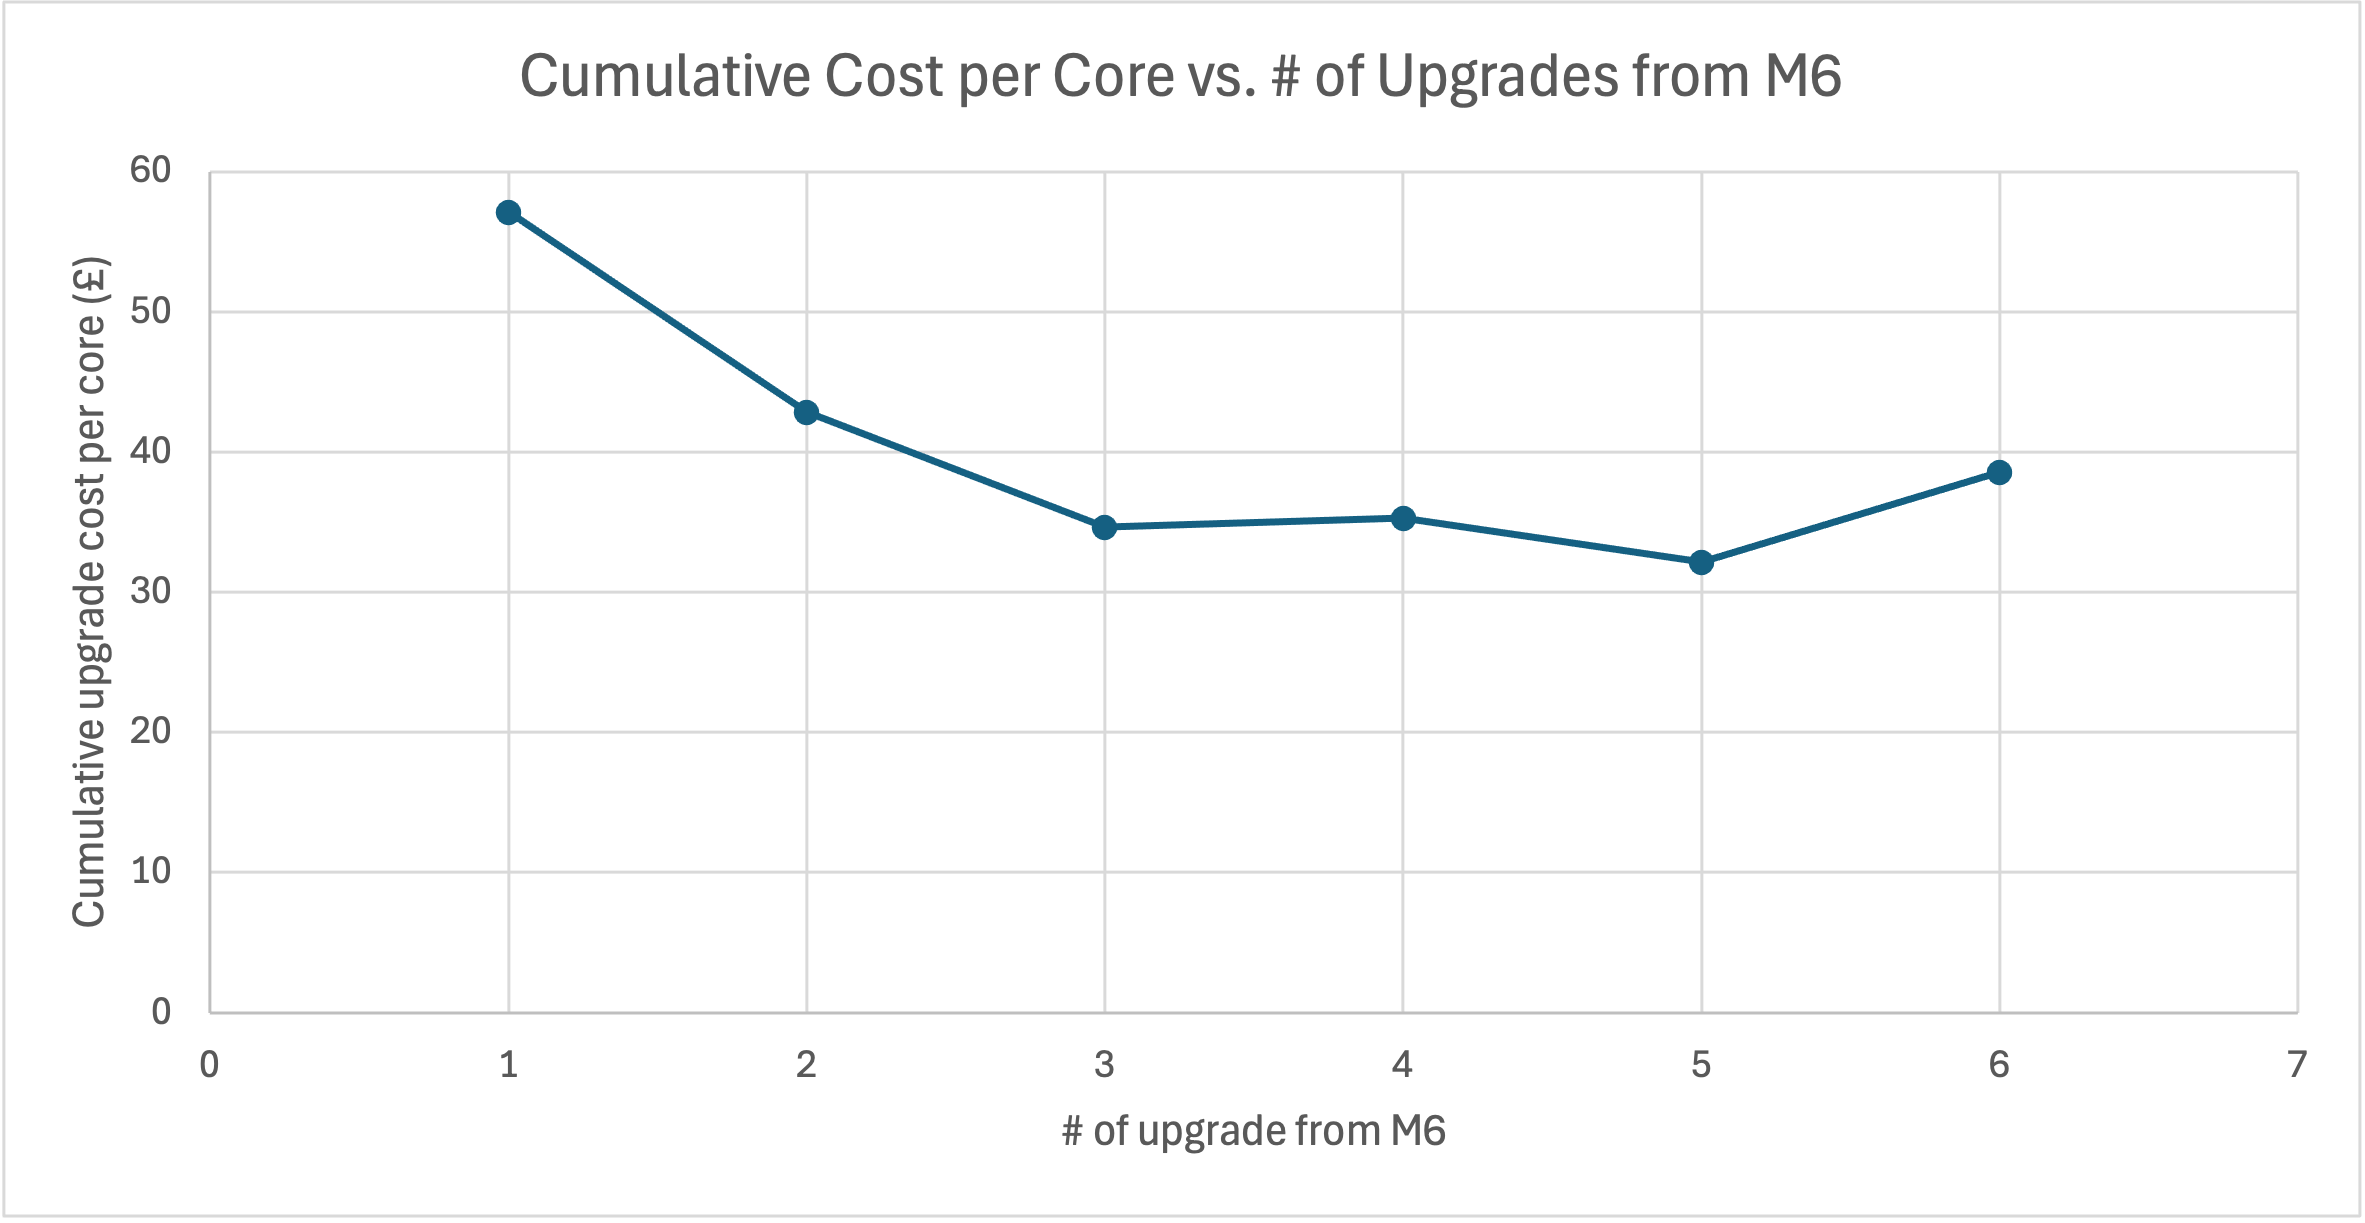
\includegraphics[width=1\textwidth]{Picture 1.png}
    \caption{Cost-per-value comparison across chips}
    \label{fig:cp-chart}
\end{figure}\\
From the Figure 1, it is clear that the most cost-effective chips, in order, are Base M5 Ultra, Base M5 Max, Maxed-out M5 Max, Maxed-out M5 Ultra, Maxed-out M5 Pro, and Base M5 Pro.
\subsection{Standard method - Performance Score}
As the number of cores increases, performance may not increase proportionally. This may be due to several factors, such as power efficiency and the architecture used. Therefore, we introduce a performance score to quantify the actual performance difference in the CPU and GPU.\\[6pt]
We apply Observations 1 and 2 to scale the price of each chip set to the same RAM and SSD storage configuration.\\[6pt]
The performance score (score) is computed using the following formula.\\
We use M6 as the base score, which is set to 1.\\
The scores of other chips are calculated using the following formula:
\begin{equation}
\text{Score}=\omega_1 d_1+\omega_2 d_2+\omega_3 d_3
\end{equation}
where\\
$w_i$ - difference between the $i$ score of a chip and M6.\\
$d_i$ - weight of the $i$ score.\\
$1$ - iGPU-FP32\\
$2$ - Geekbench 6 single-core\\
$3$ - Geekbench 6 mult-core\\[6pt]
For the standard score, we assume equal demand for the CPU and GPU; therefore, the weights are $d_1=d_2=d_3$.\\[6pt]
However, not all users place the same importance on CPU and GPU performance. Therefore, we assign different weights to single-core CPU, multi-core CPU, and GPU performance in each case, reflecting the varying priorities of different users.
\begin{table}[h]
\centering
\begin{tabular}{l|c|ccc}
\hline
Case & Type & $d_1$ & $d_2$ & $d_3$ \\
\hline
Gaming &1 & 50\% & 25\% & 25\% \\
Minecraft shaders &2& 60\% & 25\% & 15\% \\
CPU slightly focused &3& 30\% & 35\% & 35\% \\
GPU slightly focused &4 & 40\% & 30\% & 30\% \\
CPU focused &5 & 20\% & 40\% & 40\% \\
GPU focused &6 & 60\% & 20\% & 20\% \\
\hline
\end{tabular}
\caption{Weight assignments for different scenarios}
\end{table}\\
Then, we apply Equation (1) and the weights above to compute the score for all chips.
\begin{figure}[ht]
    \centering
    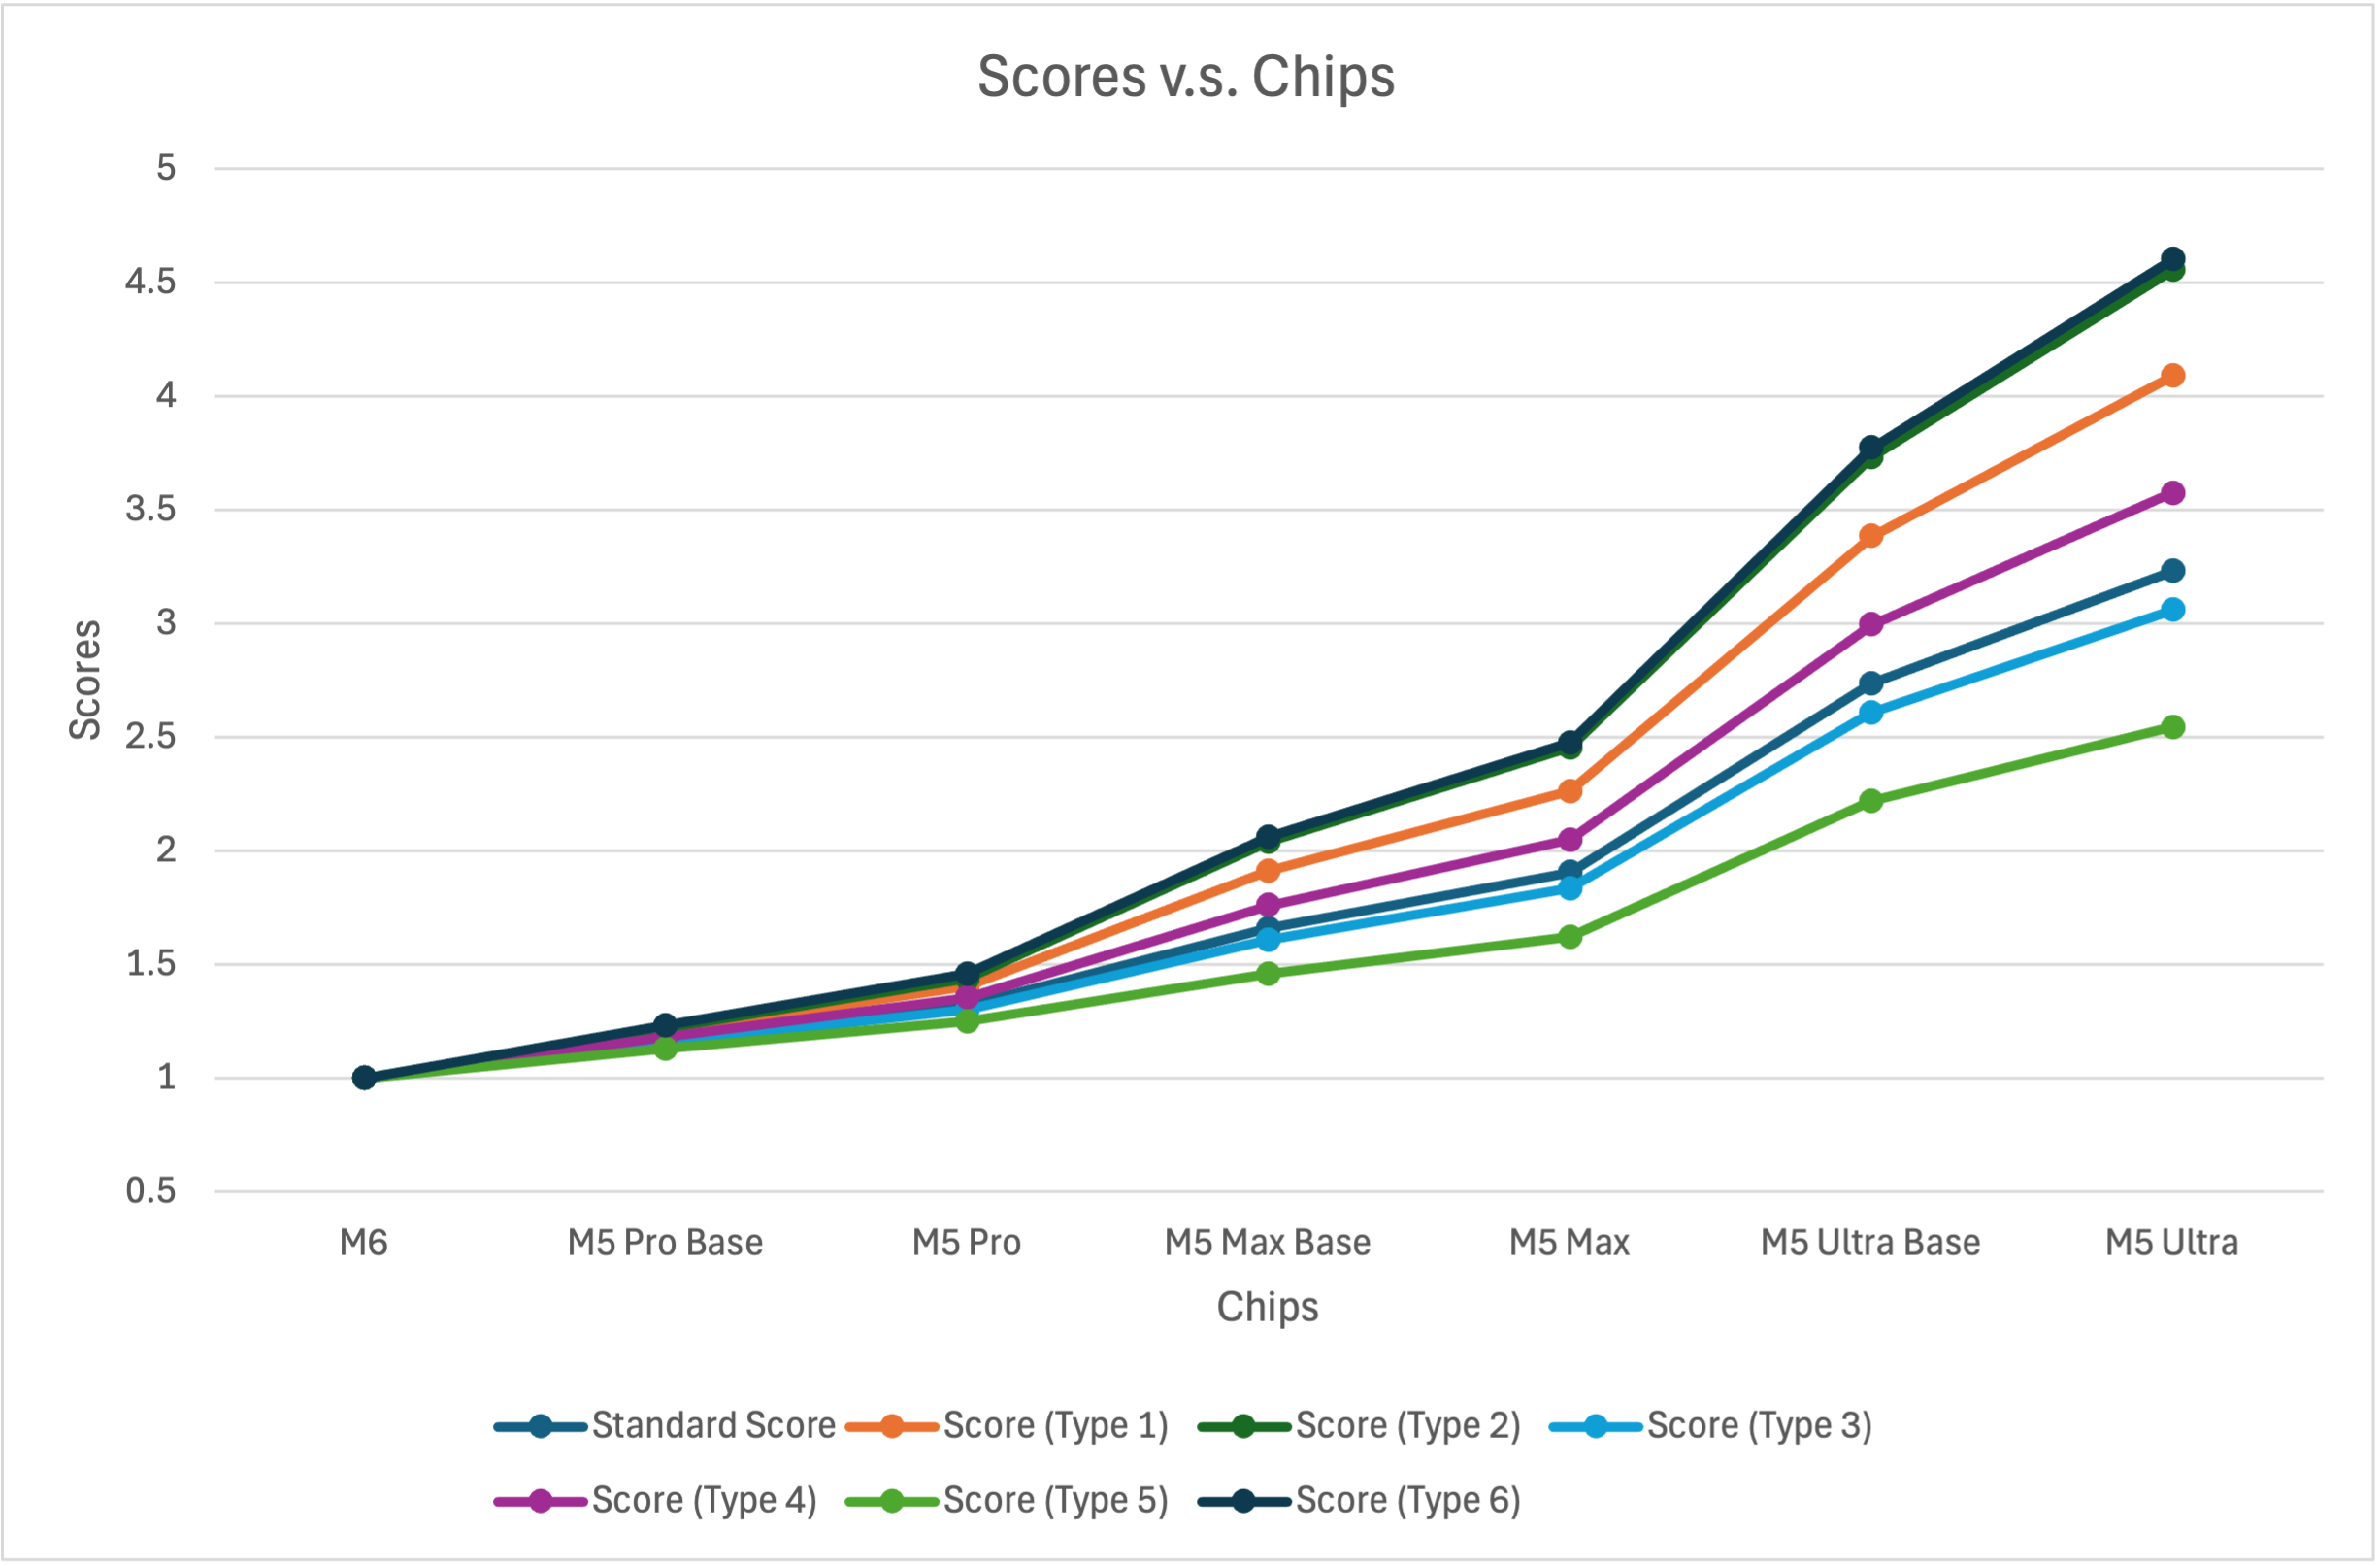
\includegraphics[width=1\textwidth]{Picture.png}
    \caption{Scores across all chips}
    \label{fig:cp-chart}
\end{figure}\\
Figure 2 shows the overall performance score pattern across all chips. It shows that the score gap between chips becomes wider as the chip tier increases, especially from M5 Max to M5 Ultra. The gradient is also steeper at the top end, which means performance improves more sharply for the higher-tier chips than for the lower ones. Depending on priority, the upgrade cost of each chip may not justify the performance gain. For example, upgrading to M5 Ultra may be more worthwhile than moving from a Base M5 Max to a Maxed-out M5 Max for CPU focused users.
\begin{figure}[ht]
    \centering
    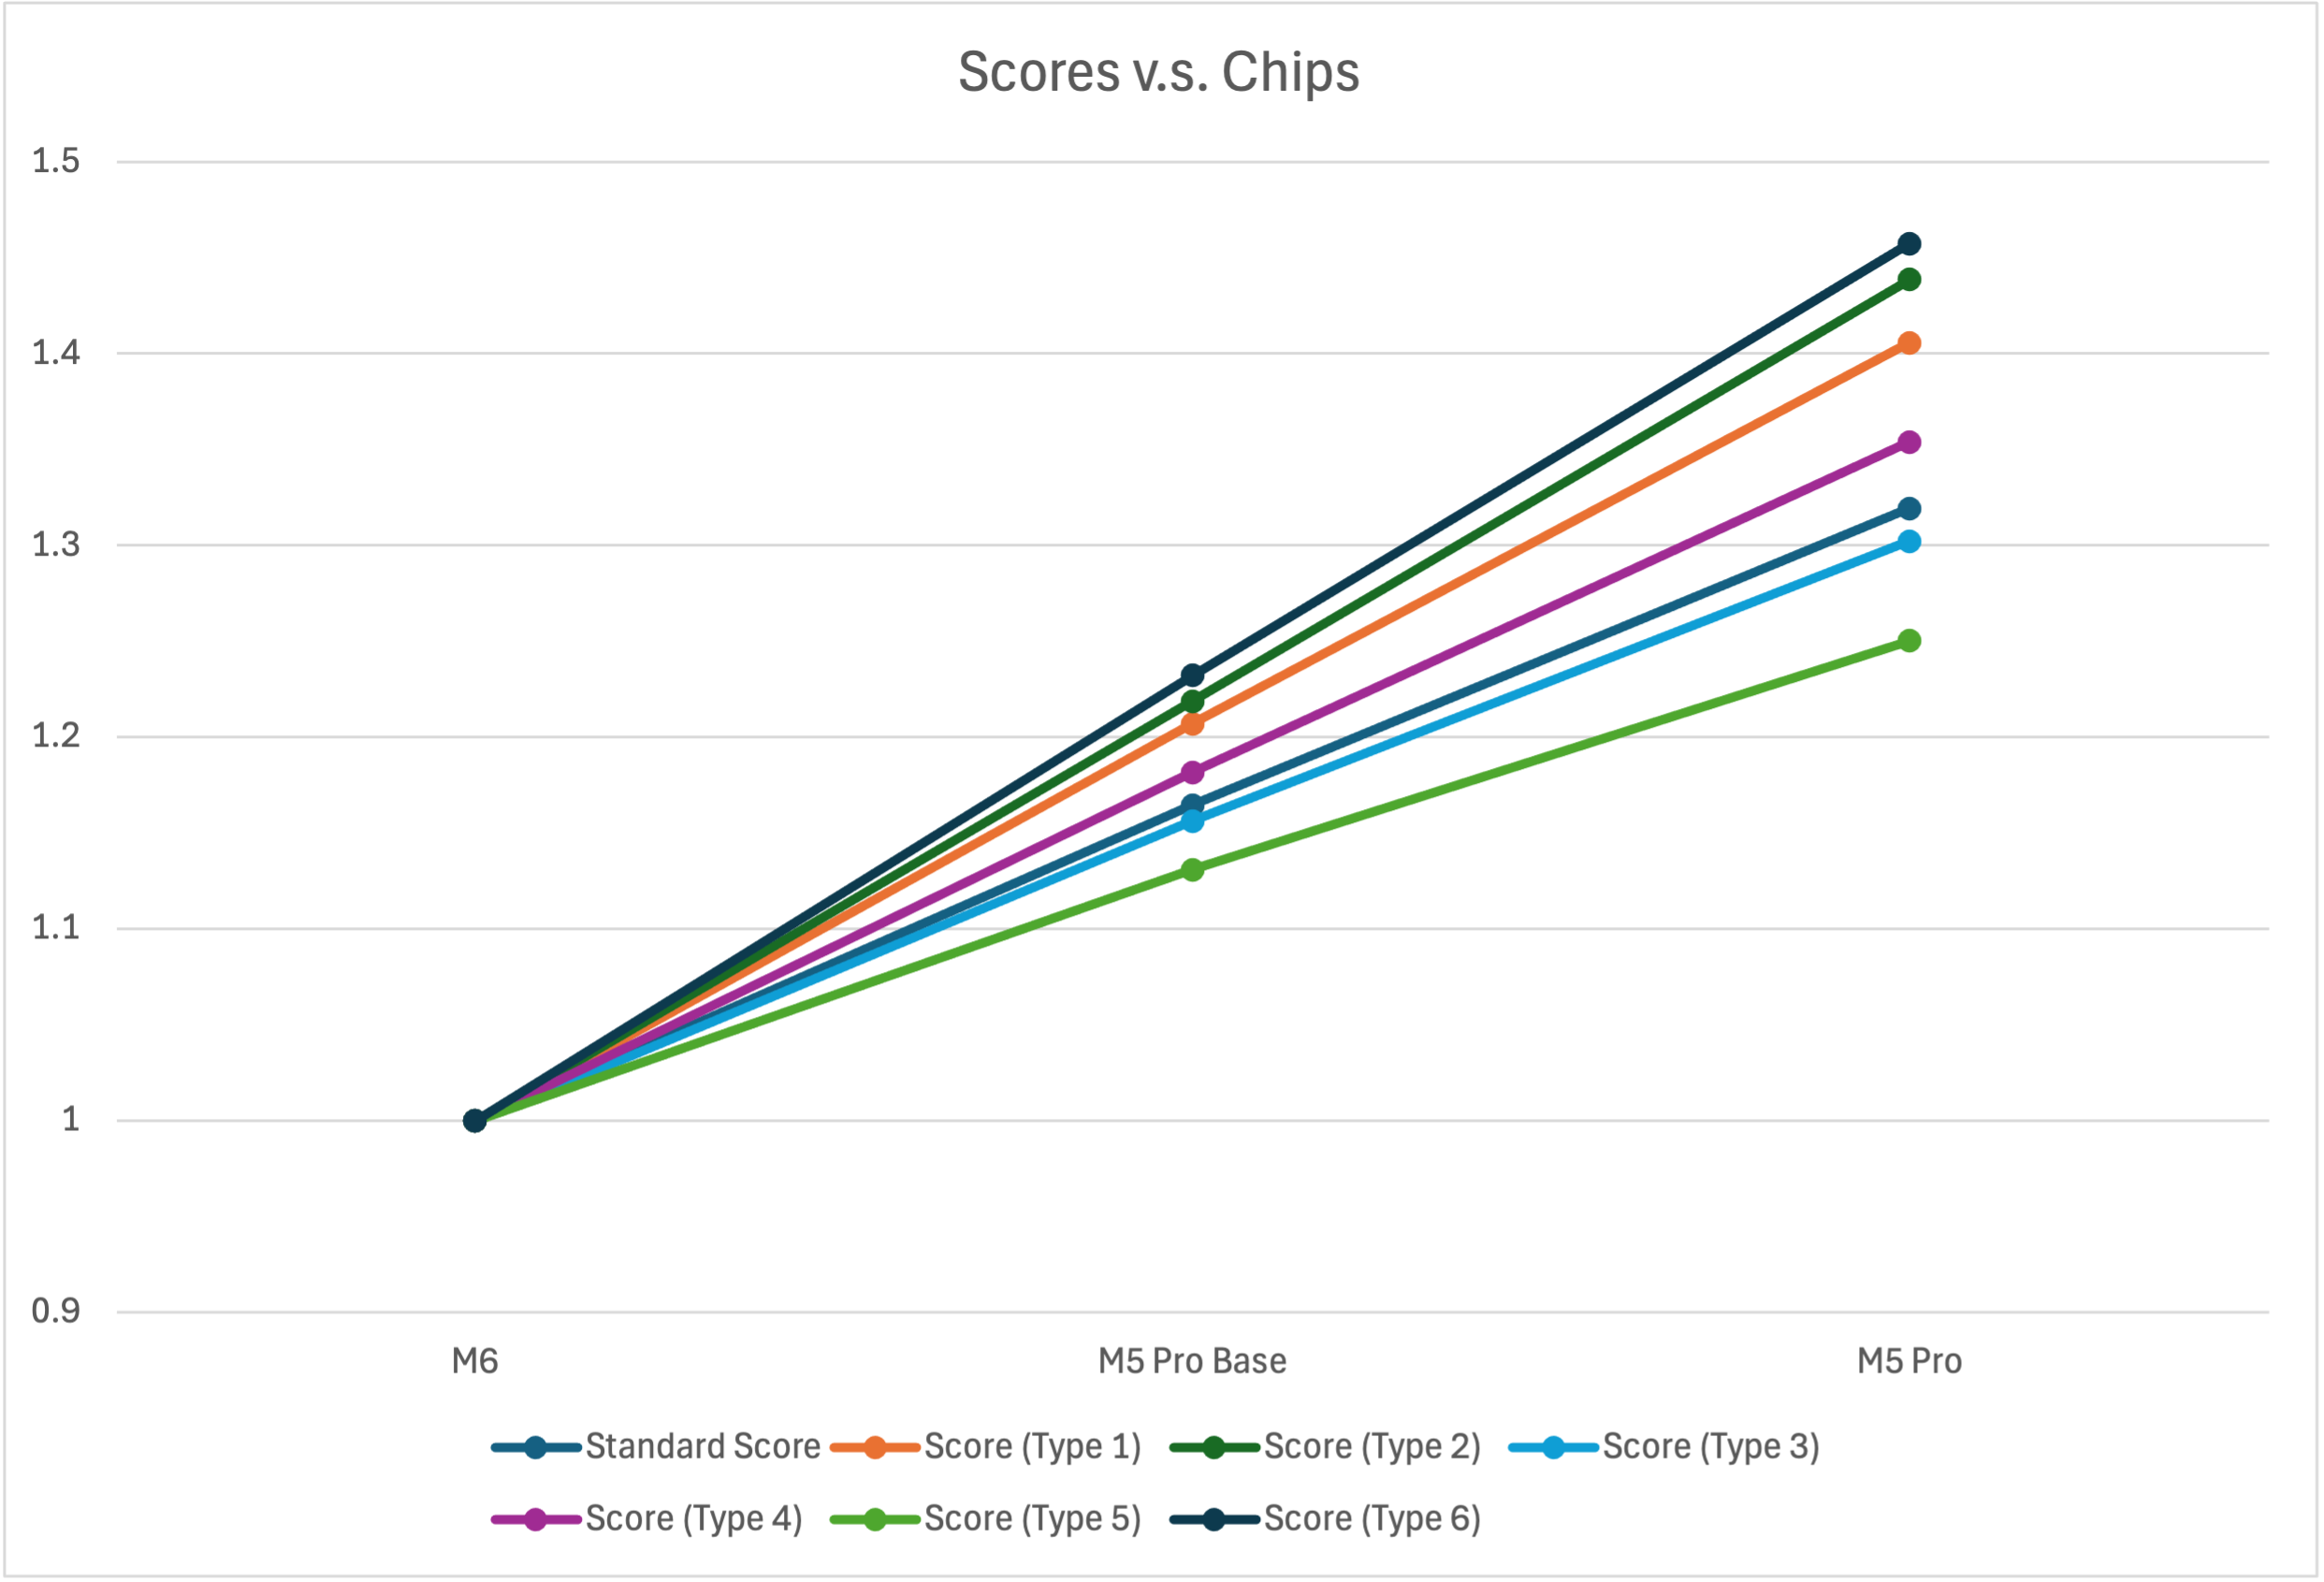
\includegraphics[width=1\textwidth]{Picture 12.png}
    \caption{Scores across M5, M5 Pro chips}
    \label{fig:cp-chart}
\end{figure}\\
As Mac Studio models are unaffordable for most people, we focus on the chips available in the Mac mini. Figure 3 narrows the comparison to the M5, base M5 Pro, and maxed-out M5 Pro chips. The figure shows a similar pattern to Figure 2. Similarly, depending on priority, the upgrade cost of each chip may not justify the performance gain. For example, for a CPU-focused user, upgrading to the base M5 Pro may be more worthwhile than upgrading to the maxed-out M5 Pro. For a GPU-focused user, the base M5 Pro and maxed-out M5 Pro may offer similar value.\\[6pt]
To answer which model is worth upgrading, we will investigate which chips have the highest cost-per-value score in the next section.
\subsubsection{Cost-Per-Value Score}
Cost-per-value score (CP score) is computed using the following formula.\\
We use M6 as the base score, which is set to 1.\\
The scores of other chips are calculated as the ratio of performance ratio to price ratio:
\begin{equation}
\text{CP score}=\frac{(\text{chip performance score}/\text{M6 performance score})}{(\text{chip price}/\text{M6 price})}
\end{equation}
The CP score reveals a completely different story from the performance score. For the standard case and Types 1, 3, 4, and 5, all M5 series chips have lower cost-effectiveness than the M6 chip. For Types 2 and 6, the only chips with a higher cost-effectiveness than M6 are the base M5 Max, maxed-out M5 Max, and base M5 Ultra.\\[6pt]
The chips with the highest cost-effectiveness are generally the M5 Max and M5 Ultra series, depending on the specific use case. For CPU-focused users, upgrading to higher-end chips tends to give lower cost-effectiveness across the upgrade path, while for GPU-focused users, certain specific chips offer better value.
\begin{figure}[ht]
    \centering
    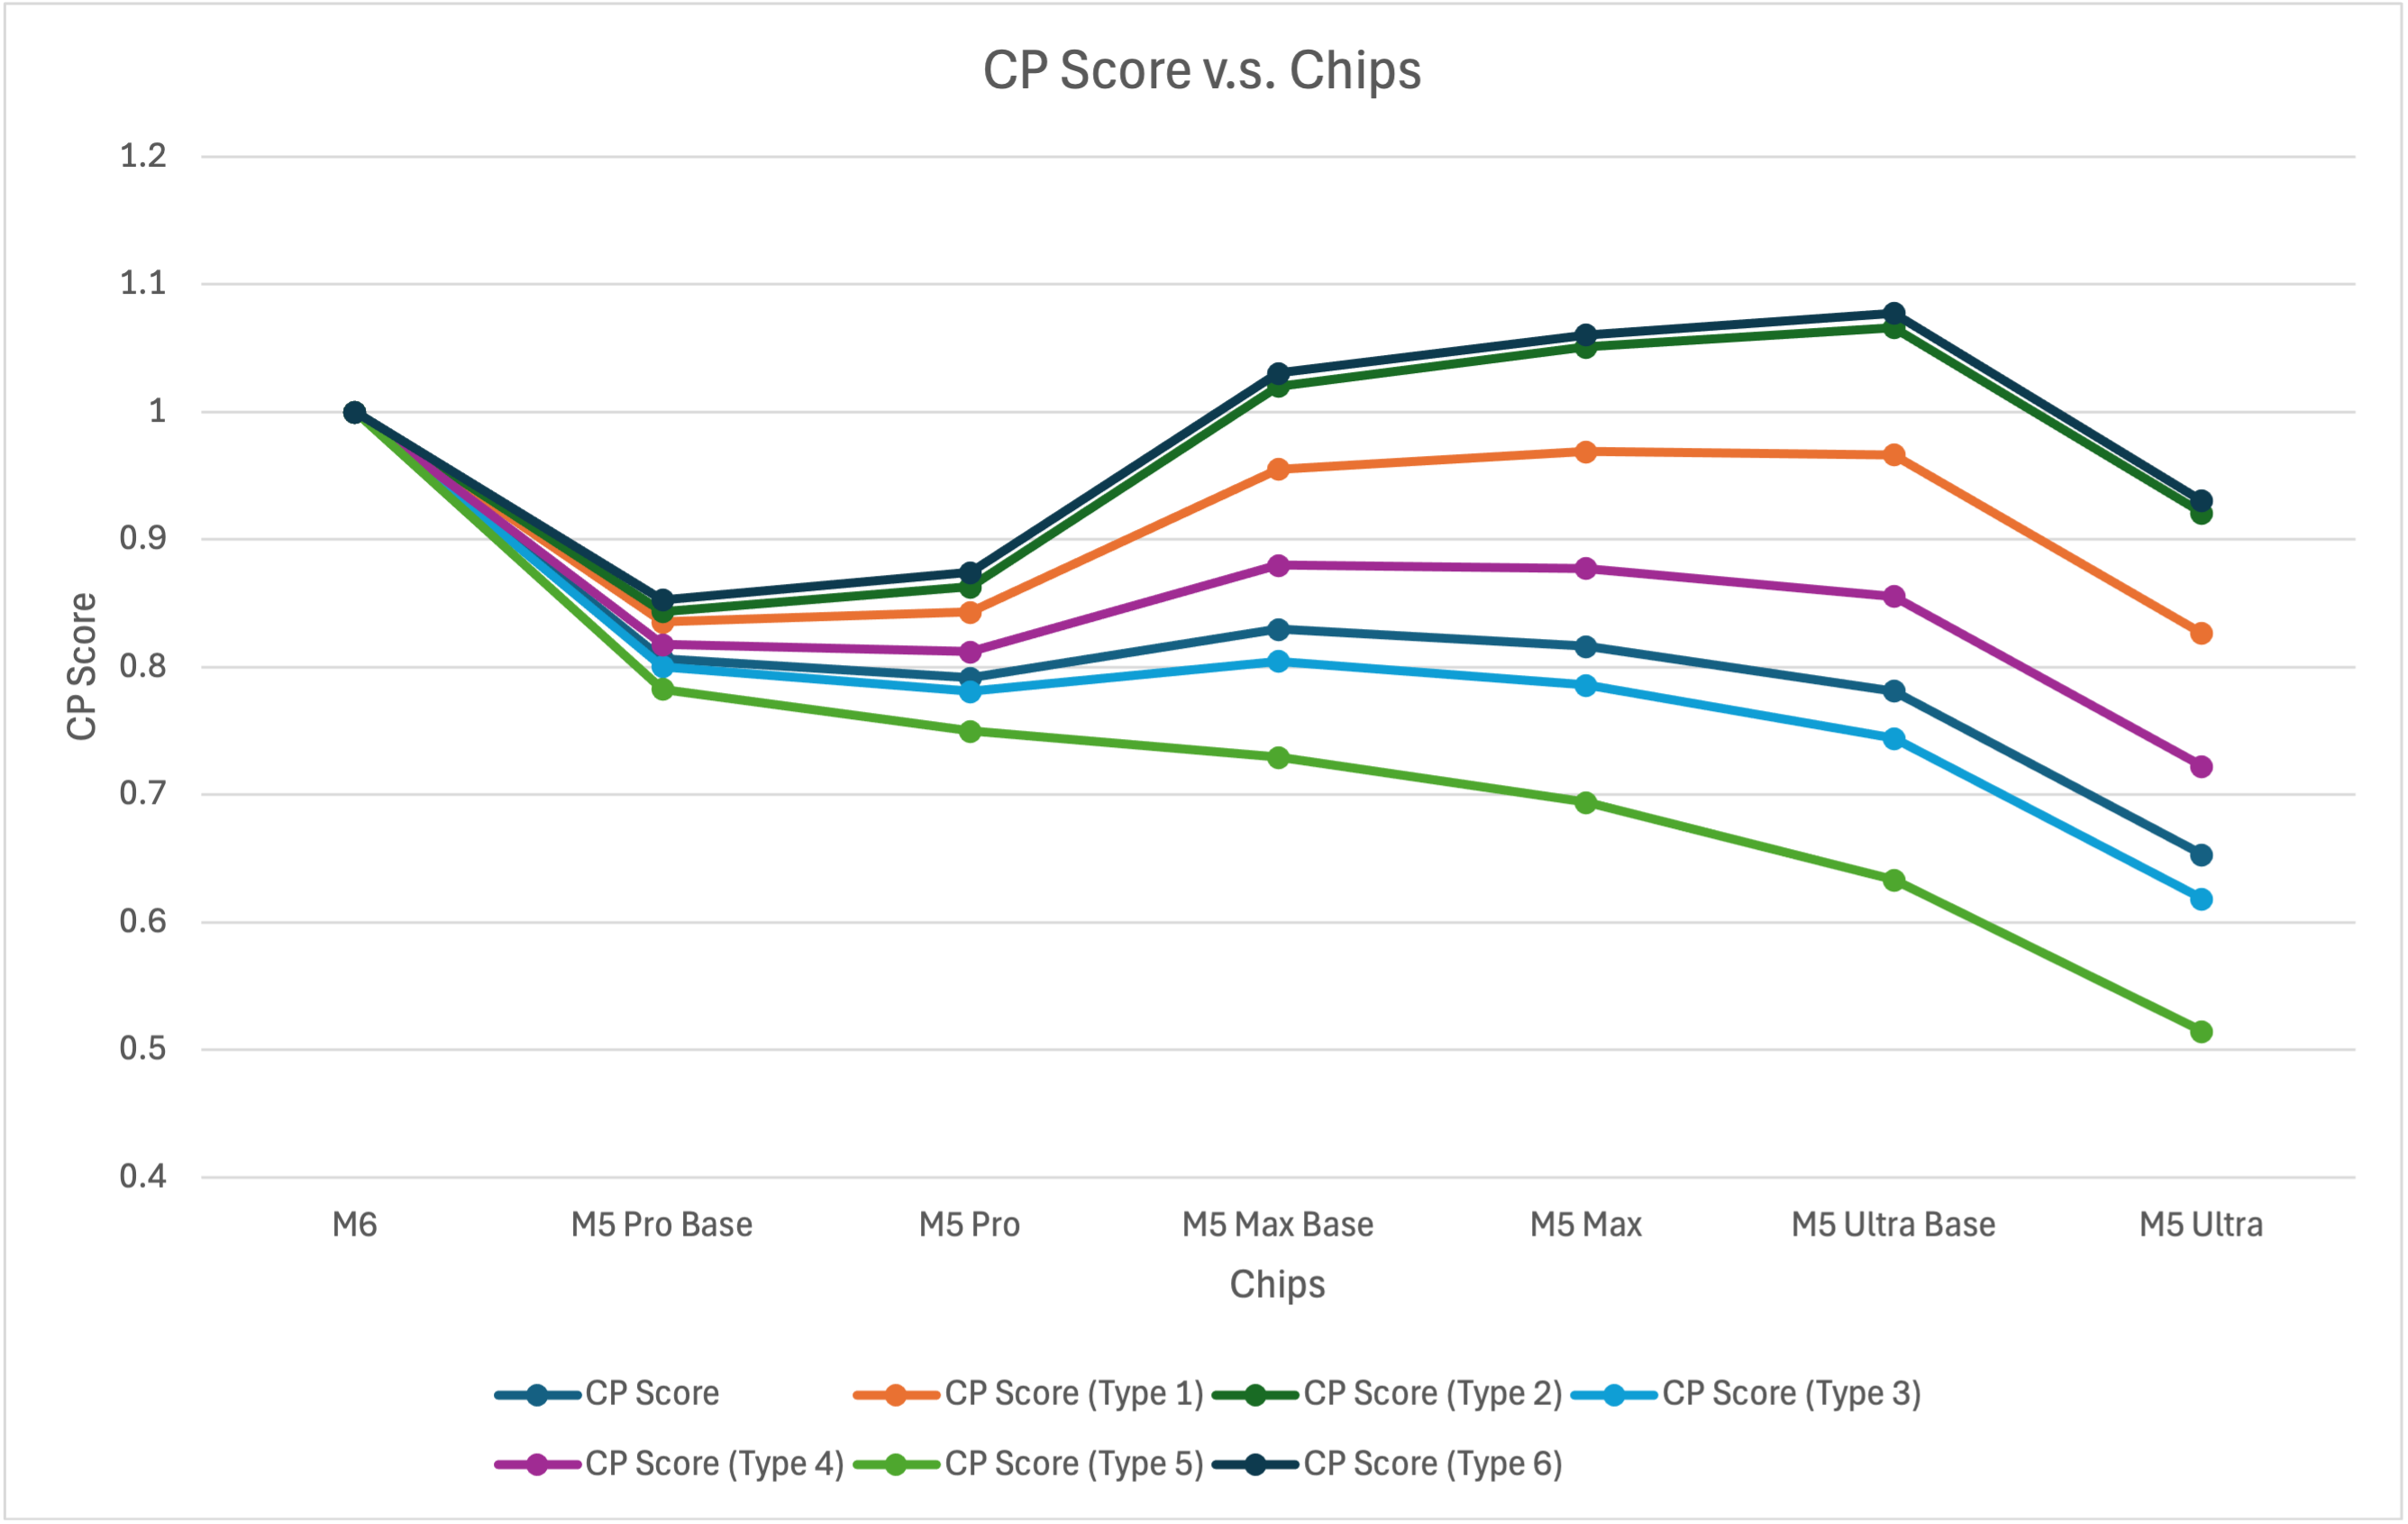
\includegraphics[width=0.95\textwidth]{Picture 155.png}
    \caption{CP Scores across all chips}
    \label{fig:cp-chart}
\end{figure}\\
If we narrow the options to M6 and the M5 Pro series, the chips with the highest cost per value are M6, followed by the M5 Pro, and then the base M5 Pro. If the user requires at least a base M5 Pro, upgrading to the M5 Pro is the more cost-efficient option.
\begin{thebibliography}{9}
\bibitem{ref1} https://nanoreview.net/en/cpu-compare
\bibitem{ref2} https://hmc-tech.com/cpus
\end{thebibliography}

\end{document}
